\documentclass[10pt,a4paper]{article}
\usepackage{fullpage}
\usepackage{amsfonts, amsmath, pifont}
\usepackage{amsthm}
\usepackage{graphicx}
\usepackage{subfig}
\usepackage{float}
\usepackage{longtable}
\usepackage{tkz-euclide}
\usepackage{titling}
\usepackage{booktabs}
\usepackage{hyperref}
\usepackage{comment}
\usepackage{tikz}
\usepackage{pgfplots}
\pgfplotsset{compat=1.13}

\setlength{\droptitle}{-7em} 
\title{CENG519 - Term Project Report}
\author{
  Cansu Eskici\\
  2588036}
\begin{document}
\maketitle
\section*{Phase 1: Ping Delay Experiment}
For this phase, I have implemented a simple processor in Python, and I conducted the experiment with 5 different delay values. 
In order to have reliable results, each value is obtained from sending the ping packets 50 times. 
On the X-axis of the chart, the numbers represent the negative power of the exponent for the lambda parameter in the random delay function, as $5e^{-x}$. For example, 3 means $5e^{-3}$, while 4 means $5e^{-4}$.


\vspace{1cm}

\begin{minipage}{0.5\textwidth}
    \begin{tikzpicture}
        \centering
        \begin{axis}[
        %title={ping-delay},
            xlabel={Mean Value For Random Delay},
            ylabel={Average RTT},
            ymin= 0, ymax = 27,
            ytick = {0,5,10,15,20,25},
            %gridstyle=dashed,
            ymajorgrids=true,
            ]
        \addplot coordinates {
          (3,23.250)(4,12.363)(5,12.056)(6,9.645)(7,9.230)
        };
      \end{axis}
    \end{tikzpicture}
\end{minipage}
\begin{minipage}{0.5\textwidth}
    \begin{table}[H]
    \centering
    \begin{tabular}{|c|c|}
        \hline
        Mean Delay Values & Mean RTT \\
        \hline
        ${5e^-3}$ & 23.250 \\
        ${5e^-4}$ & 12.363 \\
        ${5e^-5}$ & 12.056 \\
        ${5e^-6}$ & 9.645 \\
        ${5e^-7}$ & 9.230 \\
        \hline
    \end{tabular}
    \caption*{Mean Delay Values and Mean RTTs }
    \label{tab:xy_table}
\end{table}
\end{minipage}
\vspace{0.4cm}
\subsection*{Results}

The X values in the chart represent the negative power of the exponent in the random delay function,
meaning that as the value on the X axis increases, the mean delay actually decreases.
The table shows the mean delay values and the mean RTTs for each delay value.
Both the chart and the table show that the mean RTT decreases as the negative power of the exponent increases, or as the mean value for the random delay decreases.
The relationship between the mean value for random delay and the average RTT is not directly proportional.
There is a significant drop in average RTT when the negative power is increased from 3 to 4, but after 4, the differences are not as big as that.


\subsection*{Discussion}
The findings indicate that the average RTT decreases as the mean value for the random delay decreases.
Shorter delays result in shorter RTT times.
This is expected since the lower delays are likely to result in quicker packet processing and transmission.
The non-proportional relationship between the mean value for random delay and the average RTT is probably due to the exponential nature of the random delay function.
Another indicator of this is the almost indistinguishable differences among the mean RTT values with the lower mean delay values.

\section*{Phase 2: Covert Channel Implementation}
My choice of covert channel was \textit{Using options fields in TCP headers (such as timestamps) for data hiding.} 
For this purpose, I choose timestamps from TCP header options. 
This value can be used to synchronize clocks between the sender and receiver, or it can be used to measure the round-trip time of packets.
For my research, I used the following resources:
\begin{itemize}
    \item \href{https://web.mit.edu/greenie/Public/petspaper.pdf}{Covert Messaging through TCP Timestamps}
    \item \href{https://scapy.readthedocs.io/en/latest/}{Scapy Documentation}
\end{itemize}

First one is an academic paper that proposes a detailed and well structured algorithm for utilizing TCP timestamps for covert messaging. In my implementation, I did not use the same algorithm design, however it was very helpful to understand the concept of covert messaging through TCP timestamps.

The second one is Scapy documentation, I used Scapy to implement the communication between TCP client and server. 

\subsection*{Development}

For this project, I created a covert communication channel utilizing the least significant bits (LSBs) of the TCP timestamp option to encode and decode messages.


The sender encodes a given message into binary bits, splits it into chunks of a specified size (bits, meaning the number of LSBs to use per packet), and calculates a TCP timestamp value for each chunk based on its binary representation. 
Sender overwrites the least significant bits of the timestamp with this newly calculated value. 
This is done by masking out the LSBs and inserting the covert data, while the higher bits are randomized or incremented to mimic normal TCP behavior. 
Each modified timestamp is embedded in a TCP packet and sent to the receiver.
After all message bits are sent, the sender transmits a termination packet with a timestamp value of zero to signal the end of the covert message.
These timestamps are embedded in TCP packets and sent to a specified destination (dst\_ip and dst\_port). 


The receiver listens for TCP packets on the specified port and extracts the TCP timestamp value from each packet.
 For each received packet, it isolates the LSBs (using the same bit width as the sender) to recover the covert bits. 
 These bits are accumulated until the receiver observes a termination packet (timestamp value zero), at which point it reconstructs the original message from the collected bits.
  The receiver also pads the bitstream if necessary to ensure proper byte alignment before decoding.


\subsection*{Experiments}
For experimentation, the independent variables were 
\begin{itemize}
    \item \textit{Bits}, used for encoding each chunk of the message was varied across four values: 7, 8, 16, and 25.
    \item \textit{Delay}, was tested with three values: 0.01 seconds, 0.10 seconds, and 0.15 seconds.
    \item \textit{Message}, Different messages of varying lengths and content were used to test the channel's performance. The messages varied across 21, 75, 141 and 299 bytes.

\end{itemize}

The dependent variables were the average elapsed time, the capacity of the covert channel with its \%95 confidence intervals.
In order to make sure that the decoded message is correct, original message was compared with the decoded message in each experiment. 


\subsection*{Results}
\vspace{-2em}
\begin{figure}[H]
\centering
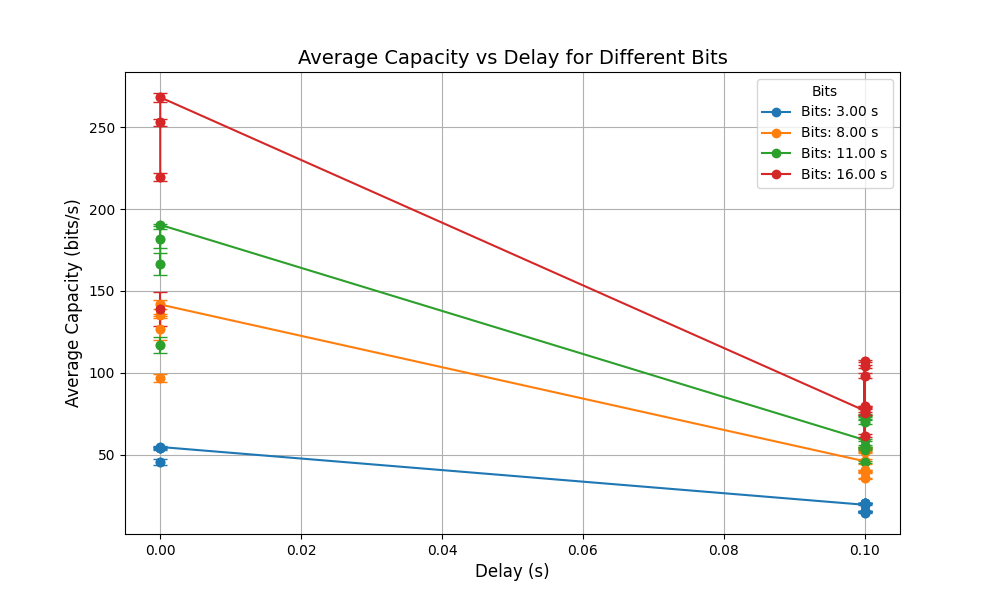
\includegraphics[width=0.8\textwidth]{capacity_vs_delay.png}


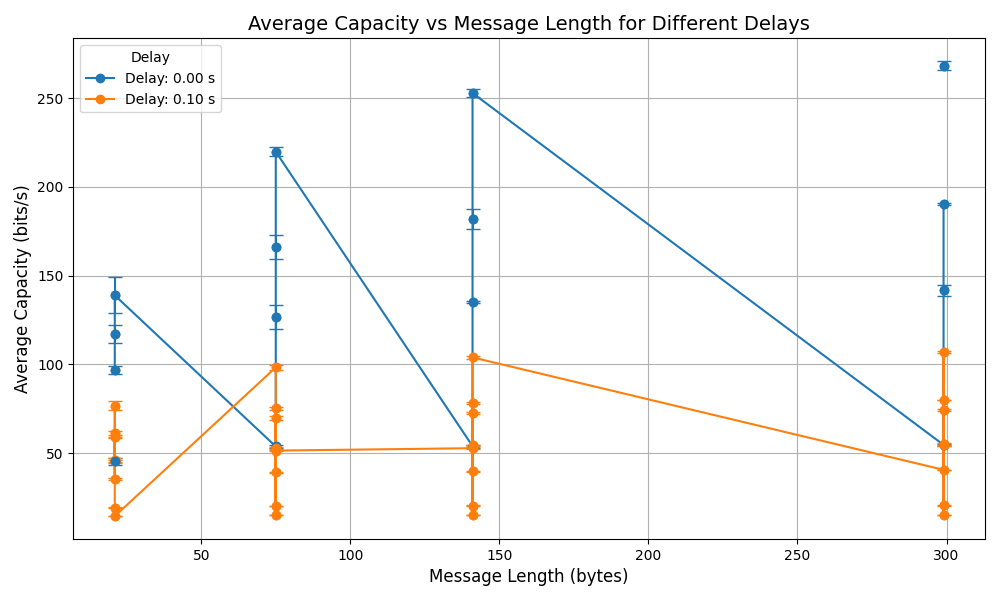
\includegraphics[width=0.7\textwidth]{capacity_vs_length.png}

\end{figure}

\begin{center}
\begin{longtable}{cccccc}
\toprule
\textbf{Bits} & \textbf{Delay (s)} & \textbf{Length (bytes)} & \textbf{Elapsed Time (s)} & \textbf{Avg Cap (bits/s)} & \textbf{Conf Interval}\\
\midrule
\endfirsthead

\multicolumn{6}{c}{} \\
\toprule
\textbf{Bits} & \textbf{Delay (s)} & \textbf{Length (bytes)} & \textbf{Elapsed Time (s)} & \textbf{Avg Cap (bits/s)} & \textbf{Conf Interval}\\
\midrule
\endhead

\midrule \multicolumn{6}{r}{{Continued on next page}} \\
\endfoot

\bottomrule
\endlastfoot

    3 & 0.05 & 21 & 3.7131 & 45.28 & [43.37, 47.19] \\ 
    3 & 0.1 & 21 & 8.7054 & 19.30 & [19.07, 19.53] \\ 
    3 & 0.15 & 21 & 11.6185 & 14.46 & [14.28, 14.64] \\ 
    3 & 0.05 & 75 & 11.1668 & 53.74 & [52.66, 54.82] \\ 
    3 & 0.1 & 75 & 29.5414 & 20.31 & [20.25, 20.37] \\  
    3 & 0.15 & 75 & 39.6026 & 15.15 & [15.09, 15.22] \\ 
    3 & 0.05 & 141 & 20.9134 & 53.94 & [53.14, 54.75] \\
    3 & 0.1 & 141 & 55.2073 & 20.43 & [20.39, 20.47] \\
    3 & 0.15 & 141 & 74.0659 & 15.23 & [15.18, 15.28] \\
    3 & 0.05 & 299 & 43.7885 & 54.63 & [53.99, 55.27]\\
    3 & 0.1 & 299 & 116.5072 & 20.53 & [20.44, 20.62] \\
    3 & 0.15 & 299 & 156.7475 & 15.26 & [15.23, 15.29] \\
    8 & 0.05 & 21 & 1.7384 & 96.66 & [94.39, 98.94] \\
    8 & 0.1 & 21 & 3.6628 & 45.89 & [44.47, 47.30] \\
    8 & 0.15 & 21 & 4.7371 & 35.47 & [35.10, 35.83] \\ 
    8 & 0.05 & 75 & 4.7400 & 126.74 & [120.09, 133.39] \\
    8 & 0.1 & 75 & 11.6741 & 51.40 & [51.10, 51.69] \\
    8 & 0.15 & 75 & 15.3037 & 39.21 & [39.00, 39.41] \\
    8 & 0.05 & 141 & 8.3356 & 135.32 & [134.66, 135.98] \\
    8 & 0.1 & 141 & 21.3806 & 52.76 & [52.35, 53.17] \\
    8 & 0.15 & 141 & 28.3113 & 39.84 & [39.55, 40.14]\\
    8 & 0.05 & 299 & 16.8828 & 141.71 & [138.74, 144.68] \\
    8 & 0.1 & 299 & 43.8644 & 54.53 & [54.25, 54.82]\\
    8 & 0.15 & 299 & 58.9632 & 40.57 & [40.53, 40.61] \\
    11 & 0.05 & 21 & 1.4358 & 117.10 & [112.19, 122.01] \\
    11 & 0.1 & 21 & 2.8537 & 58.87 & [58.39, 59.35] \\
    11 & 0.15 & 21 & 3.6916 & 45.51 & [44.90, 46.12] \\
    11 & 0.05 & 75 & 3.6108 & 166.29 & [159.54, 173.04]\\
    11 & 0.1 & 75 & 8.5973 & 69.80 & [68.64, 70.96] \\
    11 & 0.15 & 75 & 11.3469 & 52.88 & [52.50, 53.26] \\
    11 & 0.05 & 141 & 6.2000 & 182.01 & [176.45, 187.57] \\
    11 & 0.1 & 141 & 15.5720 & 72.44 & [71.76, 73.12]\\
    11 & 0.15 & 141 & 20.7125 & 54.46 & [54.18, 54.75] \\
    11 & 0.05 & 299 & 12.5631 & 190.40 & [189.67, 191.13] \\
    11 & 0.1 & 299 & 32.2634 & 74.14 & [73.57, 74.72] \\
    11 & 0.15 & 299 & 43.3510 & 55.18 & [54.79, 55.56] \\
    16 & 0.05 & 21 & 1.2120 & 138.93 & [128.78, 149.09]\\
    16 & 0.1 & 21 & 2.1883 & 76.80 & [74.44, 79.17]\\
    16 & 0.15 & 21 & 2.7382 & 61.36 & [60.46, 62.26] \\
    16 & 0.05 & 75 & 2.7289 & 219.88 & [217.39, 222.37]\\
    16 & 0.1 & 75 & 6.1037 & 98.31 & [96.88, 99.74] \\
    16 & 0.15 & 75 & 7.9808 & 75.18 & [74.39, 75.97] \\
    16 & 0.05 & 141 & 4.4596 & 252.95 & [250.72, 255.17] \\
    16 & 0.1 & 141 & 10.8522 & 103.95 & [102.96, 104.93]\\
    16 & 0.15 & 141 & 14.4513 & 78.06 & [77.55, 78.57] \\
    16 & 0.05 & 299 & 8.9140 & 268.35 & [265.73, 270.97] \\
    16 & 0.1 & 299 & 22.3323 & 107.11 & [106.44, 107.79] \\
    16 & 0.15 & 299 & 29.9707 & 79.81 & [79.65, 79.97] \\
    \end{longtable}
\end{center}
\subsection*{Discussion}

The experimental results clearly demonstrate the trade-offs inherent in the design of a TCP timestamp-based covert channel. The average capacity of the covert channel is primarily influenced by two factors: the delay and the number of bits used for encoding in each packet.
Increasing the delay between packets leads to a significant reduction in channel capacity. This is expected, as a longer delay directly limits the rate at which covert data can be transmitted. For example, with 7 bits per packet and a delay of 0.05 seconds, the average capacity is around 130--145 bits/s for longer messages, but drops to around 40 bits/s when the delay is increased to 0.15 seconds.
Increasing the number of bits encoded in each packet generally increases the channel capacity, up to a point. However, using a very large number of bits can introduce more padding and may make the channel more detectable or less robust, depending on network conditions. In the obtained results, higher bit-widths achieve capacities above 200 bits/s for short delays and long messages.
Longer messages tend to yield more stable and higher average capacities, as the overhead of setup and termination is amortized over more data. The confidence intervals for capacity also become narrower as message length increases, indicating more consistent performance.
Across all experiments, no corrupt messages were observed. The decoded messages always matched the original, demonstrating the reliability of the LSB-based covert channel under the tested conditions.


\section*{Phase 3: Covert Channel Detection}
My choice of covert channel was \textit{Using options fields in TCP headers (such as timestamps) for data hiding.} 
In this phase, I focused on detecting the covert channel that I implemented in the previous phase.  

The detection mechanism is based on analyzing the TCP header options, specifically the timestamp values.
 By monitoring the timestamp options in the TCP headers, patterns or anomalies that may indicate the presence of hidden data are identified.
  The \textit{CovertChannelDetector} class in \textit{tcp-options-processor} implements this detection logic by capturing and inspecting TCP packets for specific timestamp values that correspond to the covert channel's encoding scheme.

\subsection*{Detection Algorithm}
The detection algorithm can be summarized in the following steps:
\begin{enumerate}
    \item Capture TCP packets from the network interface.
    \item Extract the TCP header options, focusing on the timestamp values.
    \item Analyze the timestamp values for patterns or anomalies.
    \item If a potential covert channel is detected, log the details for further analysis.
\end{enumerate}

The detector passively observes TCP packets and extracts the timestamp values from the TCP options. 
It maintains a buffer of timestamp values which gets analyzed after receiving a termination signal (a timestamp value of 0).
Detection process involves analyzing the entropy of the least significant bits (LSBs) of the timestamp values. 
For each possible LSB bit, the detector computes the entropy. In a normal scenario, the entropy increases steadily as more bits are considered.
However, if a covert channel is present, the entropy will plateau or increase less rapidly at the bit width used for hiding data, since those bits are manipulated to encode the hidden message.
The \textbf{entropy-threshold parameter} is used to automatically select the optimal LSB bit width by searching for a plateau in the entropy curve, indicating the presence of a covert channel.
If a plateau is found and the entropy ratio is sufficiently low, the detector logs the timestamp values and the detected bit number, indicating the presence of a covert channel.

By this approach, the detector automatically infers both the presence of a covert channel and the number of bits used for encoding, without prior knowledge of the sender's configuration.
All detection steps are performed passively, without disrupting the normal flow of network traffic.

\subsection*{Results}

\begin{center}
\begin{longtable}{ccccc}
\toprule
Bits & Entropy & Message Length & Detector Rate & Correct Rate \\
\midrule
\endfirsthead

\multicolumn{5}{c}{{\bfseries \tablename\ \thetable{} Covert Channel Detection Results}} \\
\toprule
Bits & Entropy & Message Length & Detector Rate & Correct Rate \\
\midrule
\endhead

\midrule \multicolumn{5}{r}{{Continued on next page}} \\
\endfoot

\bottomrule
\endlastfoot

3  & 0.10 & 21  & 0.67 & 0.00 \\
3  & 0.10 & 75  & 1.00 & 0.00 \\
3  & 0.10 & 141 & 1.00 & 0.00 \\
4  & 0.10 & 21  & 1.00 & 0.00 \\
4  & 0.10 & 75  & 1.00 & 0.00 \\
4  & 0.10 & 141 & 1.00 & 0.00 \\
6  & 0.10 & 21  & 1.00 & 0.00 \\
6  & 0.10 & 75  & 1.00 & 0.00 \\
6  & 0.10 & 141 & 1.00 & 0.00 \\
8  & 0.10 & 21  & 1.00 & 0.00 \\
8  & 0.10 & 75  & 1.00 & 0.00 \\
8  & 0.10 & 141 & 1.00 & 0.00 \\
11 & 0.10 & 21  & 1.00 & 0.00 \\
11 & 0.10 & 75  & 1.00 & 0.00 \\
11 & 0.10 & 141 & 1.00 & 0.00 \\
16 & 0.10 & 21  & 1.00 & 0.00 \\
16 & 0.10 & 75  & 1.00 & 0.00 \\
16 & 0.10 & 141 & 1.00 & 0.00 \\
3  & 0.20 & 21  & 0.67 & 0.00 \\
3  & 0.20 & 75  & 1.00 & 0.00 \\
3  & 0.20 & 141 & 1.00 & 0.00 \\
4  & 0.20 & 21  & 1.00 & 0.00 \\
4  & 0.20 & 75  & 1.00 & 0.00 \\
4  & 0.20 & 141 & 1.00 & 0.00 \\
6  & 0.20 & 21  & 1.00 & 0.00 \\
6  & 0.20 & 75  & 1.00 & 0.00 \\
6  & 0.20 & 141 & 1.00 & 0.00 \\
8  & 0.20 & 21  & 1.00 & 0.00 \\
8  & 0.20 & 75  & 1.00 & 0.00 \\
8  & 0.20 & 141 & 1.00 & 0.00 \\
11 & 0.20 & 21  & 1.00 & 0.00 \\
11 & 0.20 & 75  & 1.00 & 0.00 \\
11 & 0.20 & 141 & 1.00 & 0.00 \\
16 & 0.20 & 21  & 1.00 & 0.00 \\
16 & 0.20 & 75  & 1.00 & 0.00 \\
16 & 0.20 & 141 & 1.00 & 0.00 \\
3  & 0.30 & 21  & 0.67 & 0.00 \\
3  & 0.30 & 75  & 1.00 & 0.00 \\
3  & 0.30 & 141 & 1.00 & 0.00 \\
4  & 0.30 & 21  & 1.00 & 0.00 \\
4  & 0.30 & 75  & 1.00 & 0.00 \\
4  & 0.30 & 141 & 1.00 & 0.00 \\
6  & 0.30 & 21  & 1.00 & 0.33 \\
6  & 0.30 & 75  & 1.00 & 0.00 \\
6  & 0.30 & 141 & 1.00 & 0.00 \\
8  & 0.30 & 21  & 1.00 & 0.00 \\
8  & 0.30 & 75  & 1.00 & 0.00 \\
8  & 0.30 & 141 & 1.00 & 0.00 \\
11 & 0.30 & 21  & 1.00 & 0.00 \\
11 & 0.30 & 75  & 1.00 & 0.00 \\
11 & 0.30 & 141 & 1.00 & 0.00 \\
16 & 0.30 & 21  & 1.00 & 0.00 \\
16 & 0.30 & 75  & 1.00 & 0.00 \\
16 & 0.30 & 141 & 1.00 & 0.00 \\
3  & 0.40 & 21  & 0.67 & 0.00 \\
3  & 0.40 & 75  & 1.00 & 0.00 \\
3  & 0.40 & 141 & 1.00 & 0.00 \\
4  & 0.40 & 21  & 0.33 & 0.00 \\
4  & 0.40 & 75  & 0.67 & 0.00 \\
4  & 0.40 & 141 & 1.00 & 0.00 \\
6  & 0.40 & 21  & 1.00 & 0.67 \\
6  & 0.40 & 75  & 1.00 & 0.33 \\
6  & 0.40 & 141 & 1.00 & 0.00 \\
8  & 0.40 & 21  & 1.00 & 0.33 \\
8  & 0.40 & 75  & 1.00 & 0.00 \\
8  & 0.40 & 141 & 1.00 & 0.00 \\
11 & 0.40 & 21  & 1.00 & 0.00 \\
11 & 0.40 & 75  & 1.00 & 0.00 \\
11 & 0.40 & 141 & 1.00 & 0.00 \\
16 & 0.40 & 21  & 1.00 & 0.00 \\
16 & 0.40 & 75  & 0.33 & 0.00 \\
16 & 0.40 & 141 & 0.67 & 0.00 \\
\end{longtable}
\end{center}

\subsection*{Discussion}
The results demonstrate that the entropy-based detector is highly effective at identifying the presence of a covert channel, as indicated by the consistently high detector rates (often 1.00) across all tested configurations of bit width, entropy threshold, and message length.
 This suggests that the method is robust and sensitive to the statistical anomalies introduced by covert data embedding in TCP timestamp fields.
However, the correct detection rate—representing the detector's ability to accurately infer the exact number of LSBs used for encoding—is almost always 0.00, with only a few exceptions (notably at 6 bits and higher entropy thresholds).
 This highlights a limitation of the current approach: while it reliably signals the existence of a covert channel, it struggles to precisely determine the channel's parameters. 
This is likely due to the subtlety of entropy plateaus and the inherent noise in real-world network traffic.
Trying all the possible bit widths may be possible but it is not computationally efficient.
The detector's performance suggests that while it is effective at identifying covert channels, it may require further refinement or additional heuristics to improve its accuracy in determining the specific encoding parameters used by the sender.
\newpage
\section*{Phase 4: Mitigation}
\subsection*{Mitigation Algorithm}

The mitigation mechanism implemented in the processor aims to disrupt the covert channel by probabilistically modifying the least significant bits (LSBs) of the TCP timestamp values in transit.
 For every TCP packet containing a timestamp option, the processor applies mitigation with a probability determined by the mitigation\_coef parameter.
  When mitigation is triggered, a random number of LSBs (between 0 and 4) in the timestamp value (TSval) are cleared (set to zero), and the modified timestamp is written back into the TCP options field. 
  The altered packet is then forwarded to its destination. This approach introduces controlled noise into the timestamp field, making it difficult for a covert receiver to reliably reconstruct hidden data. 
  By tuning the mitigation\_coef, the strength of the mitigation can be adjusted, allowing for a balance between normal network operation and the disruption of covert communication
  The randomization of the number of bits cleared further increases the uncertainty for any covert channel, enhancing the effectiveness of the mitigation strategy.

\subsection*{Results}

\begin{center}
\begin{longtable}{cccc}
\toprule
Bits & Mitigation Coefficient & Message Length & Receiver Correct Rate \\
\midrule
\endfirsthead

\multicolumn{4}{c}{{\bfseries \tablename\ \thetable{} Mitigation Experiment Results}} \\
\toprule
Bits & Mitigation Coefficient & Message Length & Correct Receiving Rate \\
\midrule
\endhead

\midrule \multicolumn{4}{r}{{Continued on next page}} \\
\endfoot

\bottomrule
\endlastfoot

3  & 0.01 & 21  & 0.67 \\
3  & 0.01 & 75  & 0.00 \\
3  & 0.01 & 141 & 0.00 \\
4  & 0.01 & 21  & 1.00 \\
4  & 0.01 & 75  & 0.33 \\
4  & 0.01 & 141 & 0.33 \\
6  & 0.01 & 21  & 1.00 \\
6  & 0.01 & 75  & 0.33 \\
6  & 0.01 & 141 & 0.33 \\
8  & 0.01 & 21  & 0.67 \\
8  & 0.01 & 75  & 0.67 \\
8  & 0.01 & 141 & 1.00 \\
11 & 0.01 & 21  & 1.00 \\
11 & 0.01 & 75  & 1.00 \\
11 & 0.01 & 141 & 1.00 \\
16 & 0.01 & 21  & 1.00 \\
16 & 0.01 & 75  & 1.00 \\
16 & 0.01 & 141 & 0.67 \\
3  & 0.10 & 21  & 0.00 \\
3  & 0.10 & 75  & 0.00 \\
3  & 0.10 & 141 & 0.00 \\
4  & 0.10 & 21  & 0.00 \\
4  & 0.10 & 75  & 0.00 \\
4  & 0.10 & 141 & 0.00 \\
6  & 0.10 & 21  & 0.00 \\
6  & 0.10 & 75  & 0.00 \\
6  & 0.10 & 141 & 0.00 \\
8  & 0.10 & 21  & 0.00 \\
8  & 0.10 & 75  & 0.00 \\
8  & 0.10 & 141 & 0.00 \\
11 & 0.10 & 21  & 0.00 \\
11 & 0.10 & 75  & 0.00 \\
11 & 0.10 & 141 & 0.00 \\
16 & 0.10 & 21  & 0.00 \\
16 & 0.10 & 75  & 0.00 \\
16 & 0.10 & 141 & 0.00 \\
3  & 0.20 & 21  & 0.00 \\
3  & 0.20 & 75  & 0.00 \\
3  & 0.20 & 141 & 0.00 \\
4  & 0.20 & 21  & 0.00 \\
4  & 0.20 & 75  & 0.00 \\
4  & 0.20 & 141 & 0.00 \\
6  & 0.20 & 21  & 0.00 \\
6  & 0.20 & 75  & 0.00 \\
6  & 0.20 & 141 & 0.00 \\
8  & 0.20 & 21  & 0.00 \\
8  & 0.20 & 75  & 0.00 \\
8  & 0.20 & 141 & 0.00 \\
11 & 0.20 & 21  & 0.00 \\
11 & 0.20 & 75  & 0.00 \\
11 & 0.20 & 141 & 0.00 \\
16 & 0.20 & 21  & 0.00 \\
16 & 0.20 & 75  & 0.00 \\
16 & 0.20 & 141 & 0.00 \\
3  & 0.30 & 21  & 0.00 \\
3  & 0.30 & 75  & 0.00 \\
3  & 0.30 & 141 & 0.00 \\
4  & 0.30 & 21  & 0.00 \\
4  & 0.30 & 75  & 0.00 \\
4  & 0.30 & 141 & 0.00 \\
6  & 0.30 & 21  & 0.00 \\
6  & 0.30 & 75  & 0.00 \\
6  & 0.30 & 141 & 0.00 \\
8  & 0.30 & 21  & 0.00 \\
8  & 0.30 & 75  & 0.00 \\
8  & 0.30 & 141 & 0.00 \\
11 & 0.30 & 21  & 0.00 \\
11 & 0.30 & 75  & 0.00 \\
11 & 0.30 & 141 & 0.00 \\
16 & 0.30 & 21  & 0.00 \\
16 & 0.30 & 75  & 0.00 \\
16 & 0.30 & 141 & 0.00 \\
3  & 0.40 & 21  & 0.00 \\
3  & 0.40 & 75  & 0.00 \\
3  & 0.40 & 141 & 0.00 \\
4  & 0.40 & 21  & 0.00 \\
4  & 0.40 & 75  & 0.00 \\
4  & 0.40 & 141 & 0.00 \\
6  & 0.40 & 21  & 0.00 \\
6  & 0.40 & 75  & 0.00 \\
6  & 0.40 & 141 & 0.00 \\
8  & 0.40 & 21  & 0.00 \\
8  & 0.40 & 75  & 0.00 \\
8  & 0.40 & 141 & 0.00 \\
11 & 0.40 & 21  & 0.00 \\
11 & 0.40 & 75  & 0.00 \\
11 & 0.40 & 141 & 0.00 \\
16 & 0.40 & 21  & 0.00 \\
16 & 0.40 & 75  & 0.00 \\
16 & 0.40 & 141 & 0.00 \\
\end{longtable}
\end{center}



\subsection*{Discussion}
The results indicate that the mitigation mechanism effectively disrupts the covert channel, especially at higher mitigation coefficients.
At a mitigation coefficient of 0.01, the receiver's correct message rate is relatively high, particularly for smaller message lengths and fewer bits.
 However, as the mitigation coefficient increases, the correct message rate drops significantly, indicating that the mitigation is successful in preventing the covert channel from functioning effectively.
The results also show that the effectiveness of the mitigation varies with the number of bits used for hiding data.
 For example, with 3 bits, the correct message rate is higher at lower mitigation coefficients, but it drops to zero as the coefficient increases. 
 This suggests that the covert channel is more vulnerable to disruption when fewer bits are used.
The mitigation mechanism's probabilistic nature allows for a balance between normal network operation and the disruption of covert communication.
The results demonstrate that the entropy-based detector is highly effective at identifying the presence of a covert channel, as indicated by the consistently high detector rates (often 1.00) across all tested configurations of bit width, entropy threshold, and message length.
 This suggests that the method is robust and sensitive to the statistical anomalies introduced by covert data embedding in TCP timestamp fields.



\end{document}

